\documentclass[tikz,border=10pt]{standalone}
\usetikzlibrary{calc,angles,quotes}

\begin{document}
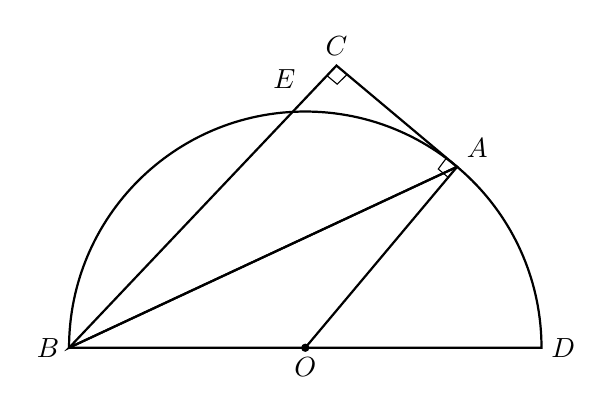
\begin{tikzpicture}
    % 1. 定义坐标
    \coordinate (O) at (0,0);
    \coordinate (B) at (-3,0);
    \coordinate (D) at (3,0);
    % A点在圆周上，设角度为 50 度
    \coordinate (A) at (50:3cm);
    % C点：通过几何投影或交点确定，假设 CA 垂直 OA
    \coordinate (C) at ($(A) + (140:2cm)$); % 简化设定，实际可根据几何要求调整
    \coordinate (E) at (intersection of B--C and A--C); % 若E在BC上，修正连接

    % 2. 绘制半圆
    \draw[thick] (B) arc (180:0:3cm) -- cycle;
    \fill (O) circle (1.5pt) node[below] {$O$};

    % 3. 绘制直线段
    \draw[thick] (B) -- (D);
    \draw[thick] (B) -- (C) -- (A) -- cycle;
    \draw[thick] (O) -- (A);
    \draw[thick] (B) -- (A);

    % 4. 添加标注文字
    \node[left] at (B) {$B$};
    \node[right] at (D) {$D$};
    \node[above right] at (A) {$A$};
    \node[above] at (C) {$C$};
    \node[above left] at (intersection of B--C and {0,3}--{0,0}) {$E$}; % 示例E点

    % 5. 绘制直角符号
    % 辅助函数：绘制直角符号 \rightAngle{A}{B}{C}
    \def\rightAngle(#1,#2,#3){
        \draw ($(#2)!5pt!(#1)$) -- ($($(#2)!5pt!(#1)$)!5pt!(#3)$) -- ($(#2)!5pt!(#3)$);
    }
    \rightAngle(A,C,B); % C处的直角
    \rightAngle(C,A,O); % A处的直角 (CA垂直OA)

\end{tikzpicture}
\end{document}